\documentclass{beamer}
\mode<presentation>
\usepackage{amsmath,amssymb,mathtools}
\usepackage{textcomp}
\usepackage{gensymb}
\usepackage{adjustbox}
\usepackage{subcaption}
\usepackage{enumitem}
\usepackage{multicol}
\usepackage{listings}
\usepackage{url}
\usepackage{graphicx} % <-- needed for images
\def\UrlBreaks{\do\/\do-}

\usetheme{Boadilla}
\usecolortheme{lily}
\setbeamertemplate{footline}{
  \leavevmode%
  \hbox{%
  \begin{beamercolorbox}[wd=\paperwidth,ht=2ex,dp=1ex,right]{author in head/foot}%
    \insertframenumber{} / \inserttotalframenumber\hspace*{2ex}
  \end{beamercolorbox}}%
  \vskip0pt%
}
\setbeamertemplate{navigation symbols}{}

\lstset{
  frame=single,
  breaklines=true,
  columns=fullflexible,
  basicstyle=\ttfamily\tiny   % tiny font so code fits
}

\numberwithin{equation}{section}

% ---- your macros ----
\providecommand{\nCr}[2]{\,^{#1}C_{#2}}
\providecommand{\nPr}[2]{\,^{#1}P_{#2}}
\providecommand{\mbf}{\mathbf}
\providecommand{\pr}[1]{\ensuremath{\Pr\left(#1\right)}}
\providecommand{\qfunc}[1]{\ensuremath{Q\left(#1\right)}}
\providecommand{\sbrak}[1]{\ensuremath{{}\left[#1\right]}}
\providecommand{\lsbrak}[1]{\ensuremath{{}\left[#1\right.}}
\providecommand{\rsbrak}[1]{\ensuremath{\left.#1\right]}}
\providecommand{\brak}[1]{\ensuremath{\left(#1\right)}}
\providecommand{\lbrak}[1]{\ensuremath{\left(#1\right.}}
\providecommand{\rbrak}[1]{\ensuremath{\left.#1\right)}}
\providecommand{\cbrak}[1]{\ensuremath{\left\{#1\right\}}}
\providecommand{\lcbrak}[1]{\ensuremath{\left\{#1\right.}}
\providecommand{\rcbrak}[1]{\ensuremath{\left.#1\right\}}}
\theoremstyle{remark}
\newtheorem{rem}{Remark}
\newcommand{\sgn}{\mathop{\mathrm{sgn}}}
\providecommand{\abs}[1]{\left\vert#1\right\vert}
\providecommand{\res}[1]{\Res\displaylimits_{#1}}
\providecommand{\norm}[1]{\lVert#1\rVert}
\providecommand{\mtx}[1]{\mathbf{#1}}
\providecommand{\mean}[1]{E\left[ #1 \right]}
\providecommand{\fourier}{\overset{\mathcal{F}}{ \rightleftharpoons}}
\providecommand{\system}{\overset{\mathcal{H}}{ \longleftrightarrow}}
\providecommand{\dec}[2]{\ensuremath{\overset{#1}{\underset{#2}{\gtrless}}}}
\newcommand{\myvec}[1]{\ensuremath{\begin{pmatrix}#1\end{pmatrix}}}
\let\vec\mathbf

\title{MatGeo Presentation - Problem 1.11.1}
\author{EE25BTECH11064 - Yojit Manral}
\date{}

\begin{document}

\frame{\titlepage}
\begin{frame}{Question}
Find a vector $\vec{r}$ that is equally inclined to the three axes and whose magnitude is $3\sqrt{3}$ units.
\end{frame}

\begin{frame}{Solution}

$\rightarrow$ A vector that subtends equal angles to all three axes will have equal components. Let the scaling factor be c. Then,\\

\begin{align}
	\text{Given that, } \norm{\vec{r}} = 3\sqrt{3} \text{ and } \vec{r} &= c\myvec{1\\1\\1} \\
	\implies \norm{\vec{r}} &= \abs{c}\norm{\myvec{1\\1\\1}} \\
	\implies \norm{\vec{r}} &= \abs{c}\sqrt{3} \\
	\implies 3\sqrt{3} &= \abs{c}\sqrt{3}\\
	\implies \abs{c} &= 3\\
    \implies \vec{r}&=\myvec{3\\3\\3} \text{ or } \vec{r}=\myvec{-3\\-3\\-3}
\end{align}

\end{frame}

\begin{frame}{Plot}
\begin{figure}[h!]
   \centering
   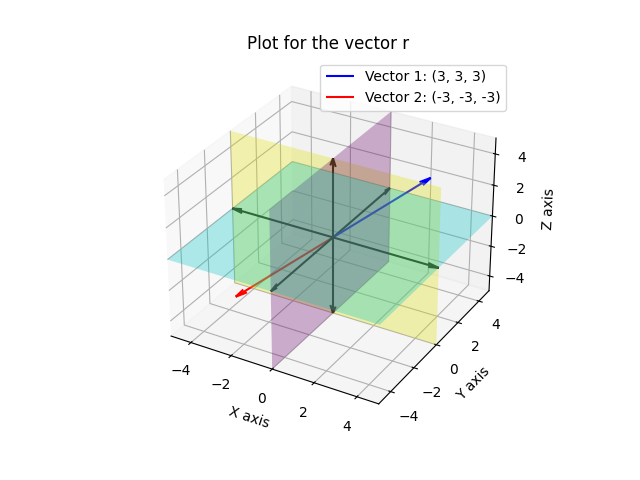
\includegraphics[width=0.8\linewidth]{figs/01.png}
   \caption{Plot of the vector $\vec{r}$}
   \label{Plot_1}
\end{figure}
\end{frame}
 % --------- CODE APPENDIX ---------
\section*{Appendix: Code}

% C program
\begin{frame}[fragile]{File: points.c}
\begin{lstlisting}[language=C]
#include <stdio.h>

int main() {
  FILE *fp;

  // -------------------
  // Question 1.11.1
  // -------------------


  fp = fopen("points.dat", "w");
  fprintf(fp, "%d,%d,%d\n", 3, 3, 3);  // 1
  fprintf(fp, "%d,%d,%d\n", -3, -3, -3);   // 2
  fclose(fp);
  return 0;
  }
\end{lstlisting}
\end{frame}

% Python calling C
\begin{frame}[fragile]{File: call\_c.py}
\begin{lstlisting}[language=Python]
import subprocess

# Compile the C program
subprocess.run(["gcc", "points.c", "-o", "points"])

# Run the compiled C program
result = subprocess.run(["./points"], capture_output=True, text=True)

# Print the output from the C program
print(result.stdout)
\end{lstlisting}
\end{frame}

% Python plotting
\begin{frame}[fragile]{File: plot.py}
\begin{lstlisting}[language=Python]
import numpy as np
import matplotlib.pyplot as plt
from mpl_toolkits.mplot3d import Axes3D

# Define the points directly
point1 = np.array([3, 3, 3], dtype=float)  # First point (3, 3, 3)
point2 = np.array([-3, -3, -3], dtype=float)  # Second point (-3, -3, -3)

# Create the figure and 3D axis
fig = plt.figure()
ax = fig.add_subplot(111, projection='3d')

# Calculate vector components for the two paths
vector1 = point1  # Vector from origin to (3, 3, 3)
vector2 = point2  # Vector from origin to (-3, -3, -3)

# Define unit vectors for the x, y, and z axes
x_axis = np.array([1, 0, 0], dtype=float)
y_axis = np.array([0, 1, 0], dtype=float)
z_axis = np.array([0, 0, 1], dtype=float)

# Plot the vectors as arrows using quiver
# Vector 1
ax.quiver(0, 0, 0, vector1[0], vector1[1], vector1[2],
          color='b', label='Vector 1: (3, 3, 3)', arrow_length_ratio=0.1)

# Vector 2
ax.quiver(0, 0, 0, vector2[0], vector2[1], vector2[2],
          color='r', label='Vector 2: (-3, -3, -3)', arrow_length_ratio=0.1)
\end{lstlisting}
\end{frame}

\begin{frame}[fragile]{File: plot.py}
\begin{lstlisting}[language=Python]
# Draw the x, y, z axes
ax.quiver(0, 0, 0, 5, 0, 0, color='black', arrow_length_ratio=0.1)
ax.quiver(0, 0, 0, 0, 5, 0, color='black', arrow_length_ratio=0.1)
ax.quiver(0, 0, 0, 0, 0, 5, color='black', arrow_length_ratio=0.1)
ax.quiver(0, 0, 0, -5, 0, 0, color='black', arrow_length_ratio=0.1)
ax.quiver(0, 0, 0, 0, -5, 0, color='black', arrow_length_ratio=0.1)
ax.quiver(0, 0, 0, 0, 0, -5, color='black', arrow_length_ratio=0.1)

# Plot the XY, YZ, and ZX planes with transparency
# Define the grid
scale = 5
xx, yy = np.meshgrid(np.linspace(-scale, scale, 10),
                     np.linspace(-scale, scale, 10))
zz = np.zeros_like(xx)
ax.plot_surface(xx, yy, zz, color='cyan', alpha=0.3, rstride=100, cstride=100)

yy, zz = np.meshgrid(np.linspace(-scale, scale, 10),
                     np.linspace(-scale, scale, 10))
xx = np.zeros_like(yy)
ax.plot_surface(xx, yy, zz, color='magenta', alpha=0.3, rstride=100, cstride=100)

xx, zz = np.meshgrid(np.linspace(-scale, scale, 10),
                     np.linspace(-scale, scale, 10))
yy = np.zeros_like(xx)
ax.plot_surface(xx, yy, zz, color='yellow', alpha=0.3, rstride=100, cstride=100)

origin = np.array([0, 0, 0])
\end{lstlisting}
\end{frame}

\begin{frame}[fragile]{File: plot.py}
\begin{lstlisting}[language=Python]
# Set the limits of the plot
ax.set_xlim([-scale, scale])
ax.set_ylim([-scale, scale])
ax.set_zlim([-scale, scale])

# Add labels for the axes
ax.set_xlabel('X axis')
ax.set_ylabel('Y axis')
ax.set_zlabel('Z axis')

# Add a title
ax.set_title('Plot for the vector r')

# Show the label for the vector
ax.legend()

# Display the plot
plt.show()
\end{lstlisting}
\end{frame}

\end{document}
